To integrate the tested subsystem, we start from integrating the Customer subsystem with the Employee Subsystem

\begin{figure}[H]
\centering
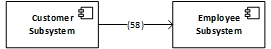
\includegraphics[scale=1]{Subsystems/Customer_employee}
\end{figure}

Then we proceed integrating the Customer subsystem with the car subsystem
\begin{figure}[H]
\centering
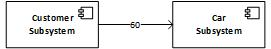
\includegraphics[scale=1]{Subsystems/Customer_car}
\end{figure}

And the other way around
\begin{figure}[H]
\centering
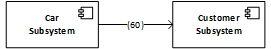
\includegraphics[scale=1]{Subsystems/Car_customer}
\end{figure}

To end the process, we integrate the Car subsystem with the employee subsystem
\begin{figure}[H]
\centering
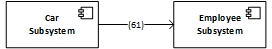
\includegraphics[scale=1]{Subsystems/Car_employee}
\end{figure}

This is the final integrated system
\begin{figure}[H]
\centering
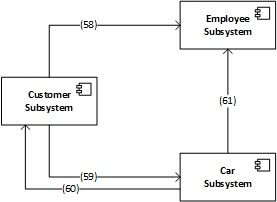
\includegraphics[scale=1]{Subsystems/Integration}
\end{figure}